\chapter{Lyapunov-based approach}

JuPE performs algorithm analysis by using the technique layed out by Van Scoy and Lessard in \cite{tutorial}. While JuPE is a blackbox tool, understanding the mathematical approach on which it is based is prequisite to understanding the package's code and functionalities.

The technique is based on the idea that certifying whether a convergence rate of an algorithm optimizing a function can be guaranteed is itself an optimization problem. This approach, which will be discussed over the sections of this chapter, 1) represents the algorithm being analyzed in state-space, 2) replaces the nonlinear gradient with constraints derived from interpolation conditions of a function class, 3) form an optimization problem using Lyapunov functions and constraints and solve it to certify whether a certain convergence rate can be guaranteed.
% The steps of this technique, which will be discussed in detail over the sections of this chapter, consists of 
% 1) viewing the algorithm as a Lur'e problem, 2) Replacing the nonlinear gradient with interpolation conditions that represent the class of smooth strongly convex functions, 3) Use lifting matrices to tighten to the interpolation condition representations, and 4) Prove whether a convergence rate is guaranteed by solving a convex semidefinte program.
%%%%%%%%%%%%%%%%%%%%%%%%%%%%%%%%%%%%%%%%%%%%%%%%%%%%%%%%%%%%%%%%%%%%%%%%%%%%%%%%
\section{Iterative algorithms as Lur'e problems}

The first step in the technique is to view optimization algorithms from a control theory perspective: As iterative gradient-based algorithms uses the gradient of the function to update \(x\), they can be reformulated into a linear time-invariant (LTI) system (how the algorithm update) in feedback with a static nonlinearity (the gradient of \(f\)) at point \(x\). Using a block diagram, the algorithm can be seen as:

\begin{figure}[h]
    \centering
	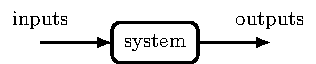
\includegraphics[width = .3 \textwidth]{block-diagram}
    \caption{Block diagram representation of iterative algorithms}
    \label{plot_block_diagram}
\end{figure}

Here, \(G\) represents the LTI system, while \(y\) and \(u\) are input and output of the gradient nonlinearity. For example, (FG) equation \ref{eqn:FG} can be rewritten to match this view as:
\begin{subequations} \label{eqn:FG2}
	\begin{align}
	  x_{k+1}     &=x_k-\alpha u_k \label{eq_FGstate},       \\
	  y_{k+1} &=x_{k+1}+\beta (x_{k+1}-x_k), \label{eq_FGinterpolated point}, \\
	  u_k &= \nabla f(y_k) \label{eq_FGggradient}
	\end{align}
	\end{subequations}
The algorithm can then be put into state-space representation with augmented state $\xi _k = (x_k, x_{k-1})$ as:
\begin{subequations} \label{eqn:FGss }
	\begin{align}
	  \xi_{k+1} &= \bmat{(1+\beta) & -\beta\\ 1 & 0}\xi_k  + \bmat{-\alpha\\ 0}u_k \label{eq_FGssstate}, \\
	  y_k &= \bmat{1+\beta & \beta}\xi_k, \label{eq_FGssinterpolation},\\
	  u_k &= \nabla f(y_k) \label{eq_FGssgradient}
	\end{align}
	\end{subequations}

It should be noted that the function $f$ is n-multivariate, and iterate $x_k$ is n-dimensional $\in \Re^n$, represented by a 1xn vector. $\xi $ therefore is a 2xn matrix.

The LTI system \(G\) can be expressed with four matrices that change in value depending on the algorithm and size depending on the number of past states used to update \(x\). For (GD), (FG), and (HB) as they are described in 1.1, these matrices are:

Beyond the three listed examples, this step can be applied to any other first order methods. Deriving an LTI system represented by matrices out of an algorithm not only creates a representation easy to understand and operate on, but also in next sections enable the representation of the past states of an algorithm and the forming of a Lyapunov function.

\section{Interpolation condition}

% For the remainder of this paper, we will focus on the only class of function currently supported by JuPE, m strong L smooth convex function \(f \in \) \(F_{m,L}\).
\subsection*{Function class interpolation conditions}

In the field of robust control theory utilized by this Lyapunov-based approach, while an LTI system is relatively simple, the nonlinearity representing the gradient of the function cannot be efficiently solved. As a result, the Lyapunov-based approach replaces the nonlinearity with a characterization of the class of function. Since the algorithm is being analyzed at discrete iterates, the characterization of a function class can be done using interpolation conditions, a set of conditions on the linearity's input and output $y$ and $u$. The interpolation conditions of a function class provide necessary and sufficient conditions under which there exists a function in that class that interpolates a given finite set of iterate-gradient pairs. These interpolation conditions depends on the characteristics of and can be derived from the function class. The interpolation condition of m strong L smooth convex functions was first formulated in \cite{taylor2016} and reformatted in \cite{tutorial} as:

\begin{theorem}[\cite{taylor2016}, Thm. 4; \cite{tutorial}, Thm. 3]
	\label{thm:interpolation_condition}
	Given index set \(I\), a set of triplets \({(y_k, u_k, f_k)}_{k \in I}\) is \(F_{m,L}-interpolable\), meaning there exists a function \(f \in F_{m,L}\) satisfying \(f(y_k) = f_k\) and \(\nabla f(y_k) = u_k\) if and only if:

	\(2(L-m)(f_i - f_j) - mL||y_i - y_j||^2 + 2(y_i - y_j)^{T}(mu_i - Lu_j) - ||u_i - u_j||^2 \geq 0\) for \(i ,j \in I\)

\end{theorem}

As an example, if we define $x_0$ as the initial iterate of an algorithm optimization a 1 strong 10 smooth convex function (\(f \in \) \(F_{1,10}\)), $\nabla f(x_0)$ as the gradient of $x_0$ at $f$, $x_s$ as the minimizer where  $\nabla f(x_s) = 0$, we can define set $I$ of \ref{thm:interpolation_condition} as including $s$ and $0$ and get the inequality:
\begin{equation} \label{eqn:int_cond}
	-20||x_0||^2 -20||x_s||^2 + 40\innerproduct{x_0}{x_s} + 22\innerproduct{\nabla f(x_0)}{x_0} - 22\innerproduct{\nabla f(x_0)}{x_s} - 2||\nabla f(x_0)||^2 \geq 0
\end{equation}
when satisfied interpolates 1 strong 10 smooth convex functions. Theorem \ref{thm:interpolation_condition} can be rewritten as:
\begin{equation} \label{eqn:int_cond2}
	% \begin{align}
	%   tr \bmat{y_i \\ y_j \\ u_i \\ u_j}^TH\bmat{y_i \\ y_j \\ u_i \\ u_j} + h^T\bmat{f_i \\ f_j} \geq 0 \\
	%   tr \bmat{y_i \\ y_j \\ u_i \\ u_j}^T\Lambda H\bmat{y_i \\ y_j \\ u_i \\ u_j} + \Lambda h^T\bmat{f_i \\ f_j} \geq 0 \\
	%   tr \Lambda \bmat{y_i \\ y_j \\ u_i \\ u_j}\bmat{y_i \\ y_j \\ u_i \\ u_j}^TH + \Lambda h^T\bmat{f_i \\ f_j} \geq 0
	\Lambda\bmat{-mL & 2mL & -mL & 2(m+L) & -2(m+L) & -2m}\bmat{||y_i||^2 \\ \innerproduct{y_i}{y_j} \\ ||y_j||^2 \\ \innerproduct{\nabla f(y_i)}{y_j} \\ \innerproduct{\nabla f(y_j)}{y_i} \\ ||\nabla f(y_j)||^2} \geq 0
	% \end{align}
\end{equation}
% With $H = \bmat{-mL & mL & m & -L\\mL & -mL & -m & L\\m & -m & -1 & 1\\-L & L & 1 & -1}$ 

%\in \Re^{6x6}%
For all $\Lambda $ such that $\Lambda_{i,j} \geq 0$. Using this equation, \ref{eqn:int_cond} can be scaled by 10 and rewritten as: \label{eqn:int_cond3}
\begin{equation} 
	\Lambda\bmat{-2 & 4 & -2 & 2.2 & -2.2 & -0.2}\bmat{||x_0||^2 \\ \innerproduct{x_0}{x_s} \\ ||x_s||^2 \\ \innerproduct{\nabla f(x_0)}{x_0} \\ \innerproduct{\nabla f(x_0)}{x_s} \\ ||\nabla f(x_0)||^2} \geq 0
\end{equation}
% The constraints on $\Lambda $ are added to the optimization problem, and the resulting nonnegative inequalities \ref{eqn:int_cond2} are combined and used in the formulation of Lyapunov functions discussed in the next section.
% Whether an algorithm being analyzed uses the gradient of multiple past states to update, or the state-space representation of an algorithm include the gradient of more than one iterate, there might exists multiple iterate-gradient pairs, each creating an inequality for their interpolation. By combining these inequalities, each scaled by a nonnegative optimization variable $\lambda $, a tight representation of the function class can be created. The inequalities in \ref{eqn:int_cond} can be combined to create:

% Basing on this theorem, [\cite{tutorial}, Cor 4] presented a non-negative linear combination of inequalities to create a tight representation of the class of function, which can be rewritten in a way easier to implement into code as:

% \begin{corollary}[\cite{tutorial}, Cor. 4]
% 	Given a function \(f \in F_{m,L}\) and let \(y_k,...,y_{k-l}\) be a sequence of iterates; \(u_{k-i} = \nabla f(y_{k-i})\) and \(f_{k-i} = f(y_{k-i})\) for \(i \in 0,...l\). Then the inequality:
	
% 	holds for all \(\Lambda \in \mathbb{R}^{(l+2) * (l+2)}\) and \(\Lambda >= 0\), and \(\Pi(\Lambda)\) and  \(\pi(\Lambda)\) are defined as:

% \end{corollary}

The left hand side of each constraint, such as \ref{eqn:int_cond2} is added to the Lyapunov functions.

\subsection*{Transpose interpolation condition}

The performance measure and the left hand side of the interpolation conditions are formulated from the norm and inner products of the state vector the end point vector, with the Lyapunov function detailed in the next section formulated using the same elements along with the gradient of the function used by the algorithm. These expressions are elements of the Gram-matrix of the vector containing every expressions the algorithm uses to update the iterates and goal vector expression. For the interpolation condition \ref{eqn:int_cond2} and a gradient descent algorithm which derive the first iterate $x_1$ using the gradient at the initial state $x_0$, the Gram matrix is:

\begin{equation} \label{eqn:trans_cond}
	\bmat{||x0||^2 & \innerproduct{xs}{x0} & \innerproduct{\nabla f(x0)}{x0} \\ \innerproduct{x0}{xs} & ||xs||^2 & \innerproduct{\nabla f(x0)}{xs} \\ \innerproduct{x0}{\nabla f(x0)} & \innerproduct{xs}{\nabla f(x0)} & ||\nabla f(x0)||^2]}	
\end{equation}

The elements of the Gram matrix are interpolable - meaning there exists vectors $x0$, $x_s$ and $\nabla f(x0)$ with which they exists, if and only if the Gram matrix is positive semidefinite. This constraint similar to those created from interpolation conditions are later added to the Lyapunov function.

\section{Lyapunov function certification}

In the final step of the Lyapunov method, Lyapunov function is created as a linear function of the state-space representation of the algorithm, an optimization variable $P$, and the constraints created by the interpolation conditions scaled by optimization variable $\lambda$. Theorem 7 proved a convergence rate can be guaranteed if there exist a $\lambda \geq 0$ and $P$ which makes the Lyapunov function nonpositive. Therefore, a minimum convergence rate can be guaranteed by solving for $P$ and $\lambda$ so that the Lyapunov function would satisfy 2 linear matrix inequalities. The mathematical basis of JuPE follows this approach with some modification. 

Define $\mathbf{x_k} = \xi _k - \xi _s $, the Lyapunov function takes the form:
% = \bmat{x_{k} - x_s \\ x_{k-1} - x_s}$, the Lyapunov function would take the form of:

\begin{equation}
	V(\mathbf{x}) = tr(\mathbf{x_k}^TP\mathbf{x_k}) \label{eqn:Lyapunov}
\end{equation}

Where $P$ is a 2x2 optimization variable. If given an algorithm with state-space representation $\xi _k$ and whose Lyapunov function satisfy the conditions:
\begin{subequations} \label{eqn:Ly_ineq}
	\begin{align}
	  ||\xi _k - \xi _s||^2 - V(\mathbf{x_k}) \leq 0,      \\
	  V(\mathbf{x_{k+1}}) - \rho ^2V(\mathbf{x_k}) \leq 0
	\end{align}
\end{subequations}

Then the convergence rate of that algorithm is guaranteed to be larger than $\rho $ for every function in the function class. While the Lyapunov function is quadratic in $\mathbf{x_k}$, due to the characteristics of matrix trace, we can see that $V(\mathbf{x})$ is linear in $\mathbf{x}^T\mathbf{x}$, reducing the inequalities to linear matrix inequalities. For gradient descent where the augmented state $\xi_k$ is just the state $x_k$, the Lyapunov function can be simplified into:
\begin{subequations}  \label{eqn:Vx}
	\begin{align*}
		V(\mathbf{x_{k}}) = tr[(x_k - x_s)^TP(x_k - x_s)]\\
						  = tr[P(x_k - x_s)(x_k - x_s)^T]\\
						  = tr[P(x_kx_k^T - x_sx_k^T - x_kx_s^T + x_sx_s^T)] \\
						  = \bmat{P & -2P & P}\bmat{||x_k||^2 \\ \innerproduct{x_k}{x_s} \\ ||x_s||^2}
	\end{align*}
\end{subequations}
Where $x_kx_s^T = x_sx_k^T = \innerproduct{x_k}{x_s}$. Similarly, $V(\mathbf{x_{k+1}})$ can be defined as:
\begin{subequations}  \label{eqn:Vx+}
	\begin{align*}
		V(\mathbf{x_{k+1}}) = V(x_k - \alpha \nabla f(x_k)) \\
						  	= tr[(x_k - \alpha \nabla f(x_k) - x_s)^TP(x_k - \alpha \nabla f(x_k) - x_s]\\
						  	= tr[P(x_k - \alpha \nabla f(x_k) - x_s)(x_k - \alpha \nabla f(x_k) - x_s)^T]\\
						  	= \bmat{P & -2P & P & 2P\alpha & -2P\alpha & P\alpha^2}\bmat{||x_k||^2 \\ \innerproduct{x_k}{x_s} \\ ||x_s||^2 \\ \innerproduct{\nabla f(x_k)}{x_k} \\ \innerproduct{\nabla f(x_k)}{x_s} \\ ||\nabla f(x_k)||^2}
	\end{align*}
\end{subequations}

The Lyapunov functions inequalities can now be completed by adding the constraints created by function class and transpose interpolation conditions. These constraints similar to the Lyapunov functions are a linear function of an optimization variable and elements of the Gram matrix. The transformation in \ref{int_con2} was done so that each nonnegative constraint is scaled by a nonnegative obtimization variable $\Lambda$, and the solver can search for $\Lambda$ just as it does for $P$ so that the linear matrix inequality is satisfied. For each constraint created by the interpolation conditions, an optimization variable $\Lambda $ is created and constrained in the optimization problem to be nonnegative if it is a scalar, nonnegative element-wise if it is a vector, or positive semidefiinite if it is a matrix. The left hand side of \ref{eqn:int_cond3} and the trace of the Gram matrix scaled by $\Lambda $ is added to both Lyapunov function. The final linear matrix inequality for gradient descent would be:

\begin{subequations} \label{eqn:Ly_ineq2}
	\begin{align*}
		\bmat{1-P-2\Lambda \\ -2+2P+4\Lambda \\ 1-P-2\Lambda \\ 2.2\Lambda \\ -2.2\Lambda \\ -0.2\Lambda}^T\bmat{||x_k||^2 \\ \innerproduct{x_k}{x_s} \\ ||x_s||^2 \\ \innerproduct{\nabla f(x_k)}{x_k} \\ \innerproduct{\nabla f(x_k)}{x_s} \\ ||\nabla f(x_k)||^2} + \Lambda tr(\bmat{||x0||^2 & \innerproduct{xs}{x0} & \innerproduct{\nabla f(x0)}{x0} \\ \innerproduct{x0}{xs} & ||xs||^2 & \innerproduct{\nabla f(x0)}{xs} \\ \innerproduct{x0}{\nabla f(x0)} & \innerproduct{xs}{\nabla f(x0)} & ||\nabla f(x0)||^2]}) \leq 0 \\
		\bmat{P-P\rho^2-2\Lambda \\ -2P+2P\rho^2+4\Lambda \\ P-P\rho^2-2\Lambda \\ 2P\alpha+2.2\Lambda \\ -2P\alpha-2.2\Lambda \\ P\alpha^2-0.2\Lambda}^T\bmat{||x_k||^2 \\ \innerproduct{x_k}{x_s} \\ ||x_s||^2 \\ \innerproduct{\nabla f(x_k)}{x_k} \\ \innerproduct{\nabla f(x_k)}{x_s} \\ ||\nabla f(x_k)||^2} + \Lambda tr(\bmat{||x0||^2 & \innerproduct{xs}{x0} & \innerproduct{\nabla f(x0)}{x0} \\ \innerproduct{x0}{xs} & ||xs||^2 & \innerproduct{\nabla f(x0)}{xs} \\ \innerproduct{x0}{\nabla f(x0)} & \innerproduct{xs}{\nabla f(x0)} & ||\nabla f(x0)||^2]}	)\leq 0
	\end{align*}
\end{subequations}

By using Lyapunov functions, we have reduced the optimization problem to a pair of linear matrix inequalities in the variables $P$ and $\Lambda$. The optimization problem can now be solved for any convergence rate $\rho$ whether there exist $P$ and $\Lambda $ so that the inequality are satisfied, proving whether $\rho$ can be guaranteed. The smallest convergence rate guarantee can be found by performing bisection search for the smallest value $\rho$ between 0 and 1 with which the optimization problem is feasible.

% By expanding \ref{eqn:xTPx}, we can see that $\mathbf{x}^T\mathbf{x}$ is a linear function of real variable, which can be transformed into a linear form. For example, for a gradient descent algorithm with step size $\alpha $ and $\xi _{k+1} - \xi _s = \bmat{x_k - \alpha * \nabla f(x_k) - x_s \\ x_k - x_s}$, we can define $o = \bmat{||x_k||^2 \\ <x_k, x_s> \\ ||x_s|| \\ ||\nabla f(x_k)||^2 \\ <\nabla f(x_k), x_k> \\ <\nabla f(x_k), x_s>}$ and $\mathbf{X}$ and $\mathbf{X^+}$as:
% \begin{subequations}  \label{eqn:X}
% 	\begin{gather}
% 		\mathbf{X}^T*o	= (\xi _k - \xi _s)^T*P*(\xi _k - \xi _s) \\
% 		\mathbf{X} = \bmat{1 & 0 & 0 & 0 & 0 & 0 \\ 0 & 1 & 0 & 0 & 0 & 0 \\ 0 & 0 & 1 & 0 & 0 & 0 \\ 0 & 0 & 0 & 0 & 0 & 0 \\ 0 & 0 & 0 & 0 & 0 & 0 \\ 0 & 0 & 0 & 0 & 0 & 0} \\
% 		\mathbf{X^+} = \bmat{1 & 0 & 0 & 0 & 0 & 0 \\ 0 & 1 & 0 & 0 & 0 & 0 \\ 0 & 0 & 1 & 0 & 0 & 0 \\ 0 & 0 & 0 & -\alpha ^2 & 0 & 0 \\ 0 & 0 & 0 & 0 & -2\alpha & 0 \\ 0 & 0 & 0 & 0 & 0 & -2\alpha}
% 	\end{gather}
% \end{subequations}

% Through this transformation, the updated state can be expressed is a linear function of $\mathbf{X}$ for any algorithm $\mathbf{X^+} = A\mathbf{X}$ where A is a real matrix. Similarly, $||\xi _k - \xi _s||^2$ can also be transformed into linear form $\mathcal{P} $ so that $\mathcal{P}^T*o = ||\xi _k - \xi _s||^2$. \ref{eqn:Ly_ineq} can now be transformed into:
% \begin{subequations} \label{eqn:newLy_ineq}
% 	\begin{align}
% 	  \mathcal{P} - tr(\mathbf{X}^TP) \leq 0      \\
% 	  tr(\mathbf{X}(A^TPA- \rho ^2P)) \leq 0
% 	\end{align}
% \end{subequations}






% \begin{equation} \label{eqn:Lyapunov}
% 	V(x) = <P, X[x; u]> = <X^T P, [x; u]>
% \end{equation}

